\section{Methods}
\label{sec:methods}

\Gls{WIPP} is a scientific workflow engine,
illustrated as shown in figure 1. This tool enables all kinds of image
visualization and analysis. Image analysis are possible thanks to the workflow
concept who enables a sequence of plugins, a piece of code put in the form of a
container, allowing all kinds of analysis or modification.

\begin{figure}[H]
  \centering
  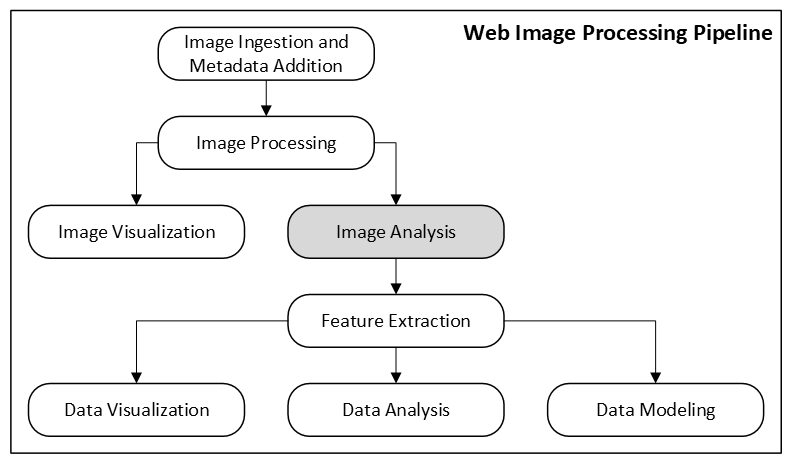
\includegraphics[width=1.0\linewidth]{png/1_wipp.png}
  \caption{\Gls{WIPP}}
  \label{fig:1wipp}
\end{figure}

Thanks to a plugin you can, for example, load an \Gls{AiModel} hosted in
\Gls{WIPP}, specify an
image collection and perform the \Gls{AiInference} of this \Gls{AiModel} on the
selected images.
The result will be a new collection of images modified by the \Gls{AiModel}, for
example
with a label after inference of a \Gls{ClassificationModel}.

\subsection{Access public \Gls{AiRepositories} via \Gls{WIPP}}

We have developed new inference plugins, see figure 2, to enable access to
\Gls{AiModel}s available on different public \Gls{AiRepositories} such as
Hugging Face \cite{HuggingFace}, BioImage.IO \cite{BioImageIo},
Cellpose \cite{Cellpose}, and more.

\begin{figure}[H]
  \centering
  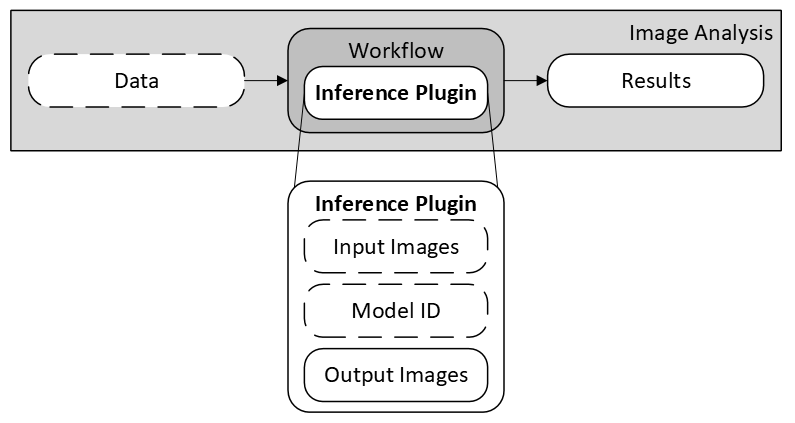
\includegraphics[width=1.0\linewidth]{png/2_inference_plugin.png}
  \caption{Inference Plugin}
  \label{fig:2inference}
\end{figure}

This was achieved by developing general-purpose code using the \Gls{API} of
the various platforms: Transformers \cite{Transformers_HuggingFace} for Hugging
Face \cite{HuggingFace}, the BioImage.IO API \cite{BioImageIoAPI} or the
Cellpose \Gls{CLI} \cite{CellposeCLI}. This
enabled us to increase the number of \Gls{AiModel}s usable
in \Gls{WIPP} thanks to containerized software.

\subsection{Document \Gls{AiModel}s}

We have introduced \Gls{AiModelCard} entries that are necessary for matching tasks
with \Gls{AiModel}s. This information will also be needed as runtime parameters.
Figure 3, training an \Gls{AI} in \Gls{WIPP} automatically generates its documentation
(\Gls{AiModelCard}).

\begin{figure}[H]
  \centering
  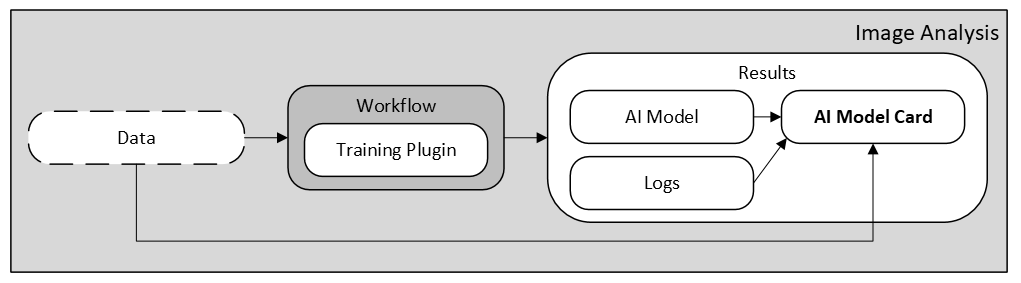
\includegraphics[width=1.0\linewidth]{png/3_ai_model_card.png}
  \caption{\Gls{AiModelCard}}
  \label{fig:3aimodelcard}
\end{figure}

This was achieved by developing code to retrieve information about the \Gls{AiModel}
throughout the pipeline: name, creation date, data used for training, number of
iterations, training time, and more.

\subsection{Compute accuracy}

We have developed a new plugin, see figure 4, to compute the \Gls{DiceIndex}.
It is a statistic used to gauge the similarity of two samples, in
our case images.

\begin{figure}[H]
  \centering
  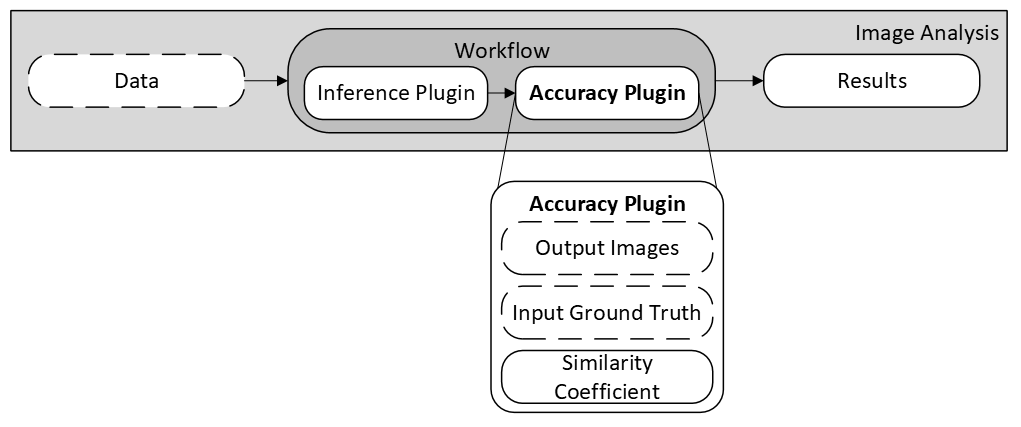
\includegraphics[width=1.0\linewidth]{png/4_accuracy.png}
  \caption{Accuracy Plugin}
  \label{fig:4accuracy}
\end{figure}

This was achieved by implementing the \Gls{DiceIndex}'s formula into a containerized
software (plugin). This makes it now possible to sequence model \Gls{AiInference} (a
model created within \Gls{WIPP} or a model from a repository) and evaluate the
accuracy of the result provided, by comparing it with
\Gls{GroundTruthData}.
